\paragraph[QuizziPedia::Front-End::ModelViews\\::QuestionsManagementModelView]{QuizziPedia::Front-End::ModelViews::QuestionsManagementModelView}

\label{QuizziPedia::Front-End::ModelViews::QuestionsManagementModelView}

\begin{figure}[ht]
	\centering
	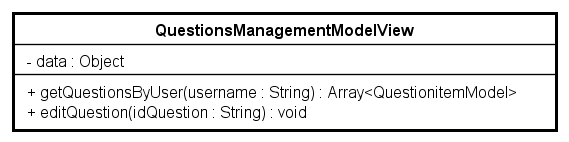
\includegraphics[scale=0.8,keepaspectratio]{UML/Classi/Front-End/QuizziPedia_Front-end_ModelView_QuestionsManagementModelView.png}
	\caption{QuizziPedia::Front-End::ModelViews::QuestionsManagementModelView}
\end{figure} \FloatBarrier

\begin{itemize}
	\item \textbf{Descrizione}: classe di tipo modelview la cui istanziazione è contenuta all'interno della variabile di ambiente \texttt{\$scope} di \textit{Angular\ped{G}}. All'interno di essa sono presenti le variabili e i metodi necessari per il \textit{Two-Way Data-Binding\ped{G}} tra la \textit{view\ped{G}} \texttt{QuestionsManagementView} e il \textit{controller\ped{G}} \texttt{QuestionsManagementController};
	\item \textbf{Utilizzo}: viene utilizzata per effettuare il \textit{Two-Way Data-Binding\ped{G}} tra la \textit{view\ped{G}} \\\texttt{QuestionsManagementView} e il \textit{controller\ped{G}} \texttt{QuestionsManagementController} rendendo disponibili variabili e metodi;
	\item \textbf{Relazioni con altre classi}: 
	\begin{itemize}
		\item \textbf{IN \texttt{QuestionsManagementView}}: \textit{view\ped{G}} contenente l’elenco delle domande create; 
		\item \textbf{IN \texttt{QuestionsManagementController}}: questa classe permette di gestire le domande create dall’utente e di crearne di nuove.
	\end{itemize}
	\item \textbf{Attributi}: 
	\begin{itemize}
		\item \texttt{- data: Object} \\ Oggetto contenete le informazioni da mostrare nell'anteprima della domanda.
	\end{itemize}
	\item \textbf{Metodi}: 
	\begin{itemize}
			\item \texttt{+ getQuestionsByUser(username: String) : Array[QuestionItemModel]} \\ 
			Metodo che acquisisce le domande create dall'utente attraverso il \texttt{QuestionService}.\\
			\textbf{Parametri}:
			\begin{itemize}
				\item \texttt{username: String} \\
				Parametro di tipo \texttt{String} contenente l'username dell'utente.
			\end{itemize}
			\item \texttt{+ editQuestion(idQuestion: String) : Void} \\ 
			Metodo che gestisce l’evento click sul pulsante per modificare la domanda. Effettua il redirect alla pagina di modifica della domanda. \\
			\textbf{Parametri}:
			\begin{itemize}
				\item \texttt{idQuestion: username} \\
				Parametro di tipo \texttt{String} contenente l'id della domanda da modificare.
			\end{itemize}
	\end{itemize}
\end{itemize}	

